\documentclass[12pt, a4paper]{article}
\usepackage{fontspec}
\usepackage{amssymb,amsfonts,amsmath}
\usepackage{ngerman}
\usepackage{booktabs}
\usepackage{microtype}

\usepackage{svg}
\usepackage{graphicx}
\graphicspath{{../img/}}

\title{Grapheigenschaften auf Kookkurrenzgraphen in Leichter und Standardsprache auf Wikipedia- und Nachrichtencorpora}
\author{Author 1, Author 2, Author 3\\Modul "`Fortgeschrittene Methoden des Information Retrieval"'}
\date{\today}

\begin{document}
\maketitle
\tableofcontents

\section{Motivation und Ziel}

áðfåéëäé¹²¤³¤’‘öó®œï¶ð߮餳€€€€

Leichte oder auch Einfache Sprache ist eine Untermenge der deutschen Sprache
die auf besonders leichte Verst\"andlichkeit optimiert ist. Sie umfasst unter
anderem spezielle Sprachregelungen, typographische Empfehlungen und
Rechtschreibregeln. 

Das \emph{Netzwerk Leichte Sprache} definiert folgende grundlegenden
Eigenschaften Leichter Sprache:

% Quellenangabe?!
\begin{itemize}
	\item Benutzen Sie einfache W\"orter
	\item Benutzen Sie W\"orter die etwas genau beschreiben
	\item Benutzen Sie bekannte W\"orter und verzichten sie auf Fachw\"orter und Fremdw\"orter
	\item Benutzen Sie immer die gleichen W\"orter f\"ur gleiche Dinge.
	\item Benutzen Sie kurze W\"orter
	\item Verzichten Sie auf Abk\"urzungen
	\item Benutzen Sie Verben
	\item Vermeiden Sie den Genitiv und Konjunktiv
	\item Vermeiden Sie Kolloquialismen und bildliche Sprache
	\item Benutzen Sie Zifferns anstatt Worten
	\item Schreiben Sie kurze S\"atze die nur eine Aussage enthalten
	\item Benutzen Sie einen einfachen Satzbau
	\item Schreiben Sie jeden Satz in eine Zeile
\end{itemize}

Das englische \"Aquivalent zu Leichter Sprache ist \emph{Simple English}. Es
existieren verschiedene Modelle des Simple English welche unterschiedliche
Ziele erreichen sollen, z.B. das \emph{Simplified Technical English}, eine
kontrollierte Sprache f\"ur technische Handb\"ucher. Aufgrund dieser
konkurrierenden Ans\"atze gibt es keine einheitliche Definition oder
Sprachpraxis des Simple English. So sind z.B. i

\section{Verwendete Technologien}
\subsection{Programmiersprache Python}

Python ist eine schreckliche Programmiersprache mit viel zu wenig geschweiften
Klammern.

\subsubsection{Natural Language Toolkit}

Das NLTK ist ein generelles Framework f\"ur Sprachverarbeitung in Python.

\subsubsection{Graphen-Bibliothek graph-tool}

graph-tool ist ein Python-Modul welches der Manipulation und statistische
Auswertung von Graphen dient. Es stellt im Kern ein C++-Wrapper um die Boost
Graph Library dar wodurch eine \"ahnliche Performanz zu nativen C-Bibliotheken
erreicht wird. Es ist zus\"atzlich in der Lage Graphen mit modernen Techniken
zu visualisieren und \"ubliche Ma\ss{}e wie Clustering-Koeffizienten, Knoten-
und Kantengrade und Durchmesser zu berechnen.

\section{Datenbasis}

Als Datenbasis wurden Quellen gew\"ahlt die sich durch eine gro\ss{}e
semantische und logische N\"ahe auszeichnen, namentlich Nachrichtenseiten in
deutscher und die Wikipedia in englischer Sprache.

\subsection{Nachrichtenseiten}

\subsubsection{nachrichtenleicht.de}

Nachrichtenleicht ist ein Dienst des Deutschlandfunks welcher einmal
w\"ochentlich die wichtigsten Nachrichten der vorangegangenen Woche in leichter
Sprache zusammenfasst. Er soll die mehreren Millionen Menschen in Deutschland
erreichen welche aus verschiedenen Gr\"unden von konventionellen
Nachrichtenangeboten ausgeschlossen sind.

\subsubsection{deunews2010\_100K-Korpus}

Als korrespondierende Datenquelle in Standardsprache wurde der
deunews\-2010\_100K-Korpus des Lehrstuhls f\"ur automatische Sprachverarbeitung
der Universit\"at Leipzig gew\"ahlt. Dieser weist eine \"ahnliche Satzzahl zu
den von nachrichtenleicht extrahierten Text aus und wurde bereits von der ASV
normalisiert.

\subsection{Wikipedia}

Die zweite Datenquelle sind Artikel aus der Wikipedia in \emph{Standard} und
\emph{Simple English}. Mit fast 120000 Lemmata stellt die Simple English
Wikipedia eine der gr\"o\ss{}ten \"offentlich verf\"ugbaren, freien
Textsammlungen in leichter Sprache dar. Zus\"atzlich ist sie die einzige
welche Dokumentenalignment aufweist.

\section{Workflow}
\subsection{Extraktion der Korpora}

Die selbsterstellten Textcorpora wurden mittels selbstgeschriebener Crawler
heruntergeladen. Nachrichtenleicht wurde rekursiv von der Startseite gequeriet
und die resultierenden Seiten in einer MongoDB gespeichert. 

Die beiden Wikipedias wurden \"uber eine Simple English Artikelliste
heruntergeladen und in einer JSON-Datei inklusive Wiki Markup gespeichert. Das
Entfernen des Markups stellte sich als eine nichttriviale Aufgabe dar. Nach
negativen Erfahrungen mit einem vollst\"andigen Parser\footnote{MediaWiki
Parser from Hell (http://mwparserfromhell.rtfd.org)} ohne und mit Kombination
von regul\"aren Ausdr\"ucken wurde ein Ansatz gew\"ahlt der nur mit regul\"aren
Ausdr\"ucken zufriedenstellende Ergebnisse erzielt. Nach Entfernen des Wiki
Markups wurden die Artikel jeweils auf die L\"ange des k\"urzeren beschnitten
und anschliessend in einer MongoDB gespeichert.

\subsection{Berechnung Kookkurrenzen}

Die Kookkurrenzen wurden von mittels der Pipeline des Lehrsstuhls f\"ur
Automatisches Sprachverarbeitung berechnet.

\subsection{Erstellung der Graphen}

Die errechneten Kookkurrenzen wurden in graph-tool-Objekte geparst. Subgraphen
aus den Korpora wurden mittels eines \emph{force-directed graph} nach
\cite{Hu2005} gelayoutet, Histogramdaten wurden aus aus graph\_tool nach R
exportiert und mittels ggplot2 geplottet.

\subsection{Berechnung von Graphen-Kenngr\"o\ss{}en}

Nach Erstellung der Graphen wollen wir sie auf typische Kenngrößen untersuchen
und anhand dieser charakterisieren und paarweise vergleichen. Für die
verschiedenen Eigenschaften bietet \texttt{graph\_tool} bereits implementierte
Algorithmen an, die wir verwenden wollen. Im Folgenden werden die Kenngrößen
kurz erläutert, unsere Erwartungen dargestellt und die Ergebnisse gezeigt.

\paragraph{Gr\"o\ss{}e (Anzahl Nodes)}
Schon in der Größe der Graphen sollten sich paarweise Unterschiede erkennen
lassen. So sollten die beiden Corpora in einfacher Sprache wesentlich weniger
verschiedene Wörter enthalten. So werden \emph{schwierige} Wörter
typischerweise durch leichter verständliche ersetzt und kommen so im einfachen
Corpus nicht vor. Die Anzahl der Knoten lässt sich natürlich trivial zählen.
Der \emph{deunews2010\_100K-Corpus} hat TODO Knoten,
\emph{nachrichtenleicht.de} TODO, die englische Wikipedia TODO, und die
\emph{simple english} Wikipedia TODO Knoten. Wir können hier erkennen, dass
.....TODO....(erwartung erfüllt?)
 
\paragraph{Kantengewichte (Histogramm)}
machen wir sowas? was sagt das aus?

\paragraph{Dichte}
Die Dichte eines Graphen beschreibt das Verhältnis von vorhandenen Kanten zu
potentiell möglichen Kanten in einem Graphen. Ein Wert von 1 bedeutet, dass
jeder Knoten mit jedem anderen Verbunden ist, dem gegenüber eine 0, dass keine
Kanten vorhanden sind. Die Dichte wird wie folgt berechnet:

\begin{center}
  \begin{math}
    \frac{|E|}{|V|(|V|-1)}
  \end{math}
\end{center}


|E| ist die Anzahl der Kanten, |V| die Anzahl der Knoten im Graphen. 

TODO: ist es hier plausibel, dass die einfachen sprachen dichter sein sollten?
es gibt ja (hoffentlich) weniger wörter, und diese wenigen sollten
dementsprechend häufiger verwendet werden und sich untereinander so leichter
verknüpfen.

\paragraph{Clusterkoeffizient}
Eng mit der Dichte verwandt ist der Clusterkoeffizient. Er beschreibt die
Anzahl vorhandener Dreiecke im Graph im Verhältnis zu möglichen Dreiecken. Drei
Knoten, die jeweils paarweise verbunden sind, bilden ein Dreieck. Ziel ist ein
Messwert der Aussagt wie sehr die Knoten Cliquen bilden. Lokal betrachtet
bedeutet der Wert die Wahrscheinlichkeit die Nachbarn eines Nachbarn zu kennen.
Da wir die Graphen global miteinander vergleichen möchten verwenden wir den
globalen Clusterkoeffizienten \emph{C}. Er berechnet sich wie folgt:

\begin{center}
  \begin{math}
    C = \frac{3*\text{Anzahl der Dreiecke}}{\text{Anzahl verbundener Tripel}}
  \end{math}
\end{center}


Ein Tripel bezeichnet drei miteinander Verbundener Knoten, nicht
notwendigerweise ein Dreieck. Knoten A kann mit Knoten B und C verbunden sein,
während B nicht mit C verbunden ist. In \emph{Small-World-Graphen} ist dieser
Wert typischerweise hoch. 


% wir können für ausgewählte wörter vielleicht noch lokale clusterkoeffizienten
% berechnen, vielleicht für die besonders hoch verbundenen? sollten diese dann
% relativ klein sein? weil hubs ja verschiedene "teilgraphen" miteinander
% verbinden

% \paragraph{(Pseudo-)Diameter}
% \paragraph{K\"urzeste Wegl\"ange}
% die beiden fasse ich im folgendem punkt zusammen

\paragraph{Wegl\"angen}
Um Small-World-Eigenschaften nachzuweisen ist ausserdem interessant die
Weglängen im Graphen zu untersuchen. Eine gute Kenngröße ist der Durchmesser
des Graphen, also der längste kürzeste Weg zwischen zwei Knoten. In einer
\emph{small-world} sind alle Knoten von allen Anderen in wenigen Schritten
erreichbar, typischerweise in höchstens 5 bis 7 Schritten. \texttt{Graph\_tool}
erlaubt zum einen die Ausgabe eines Durchmessers, wie oben beschrieben, zum
Anderen die Ausgabe eines Histogramms, welches die Vorkommen der Längen aller
kürzesten Wege zeigt.

TODO Tabelle

TODO, folgenden abschnitt an tatsächliche ergebnisse anpassen In der Tat können
wir die Schrittzahl bestätigen, beispielsweise für den
\texttt{nachrichtenleicht.de} Corpus haben wir einen Durchmesser von 6, und von
allen paarweisen Pfaden kommt dieser sogar sehr selten vor. Bei XXX Knoten gibt
es YYY Pfade zu berechnen. Die meisten Knoten sind in drei bis vier Schritten
miteinander verbunden.

                             
\paragraph{Skalenfreiheit}
skalenfrei bedeutet, dass es einige hubs mit theoretisch unendlich vielen
nachbarn gibt, die anderen knoten haben relativ wenige nachbarn. power law
verteilung entfernt man einen(mehrere) hub bricht das netzwerk schnell
auseinander. haben wir so etwas? wir können das mit graph\_tool über die
clustering algorithmen leicht ausrechnen!  skalieren die graphen paarweise um
ein paar knoten, oder kommen neue wichtige (hubs) wörter hinzu?

\paragraph{Small World Eigenschaften}
Zusammengefasst zeichnen sich Small-World-Graphen durch kleine Durchmesser und
hohe Clusterkoeffizienten aus. Skalenfreiheit ist nicht zwangsläufig wichtig!
Wir konnten sowohl die kurzen Weglängen, als auch hohe Clusteringkoeffizienten
für alle Graphen nachweisen. TODO passt das? skalenfreiheit? 


\paragraph{Übersichtstabelle}
\section{Ergebnisse}
\subsection{Weitere Beobachtungen}
\paragraph{H\"aufigste W\"orter nach Sprache}

%%%%%%%%%%%%%%%%%%%%%%%%%%%%%%%%%%%%%%%%%%%%%%%%%%%%%%%%%%%%%%%%%%%%%%%%%%%%%%%%
\section{Testkapitel mit Testgrafiken}

\subsection{pdf-Grafik}
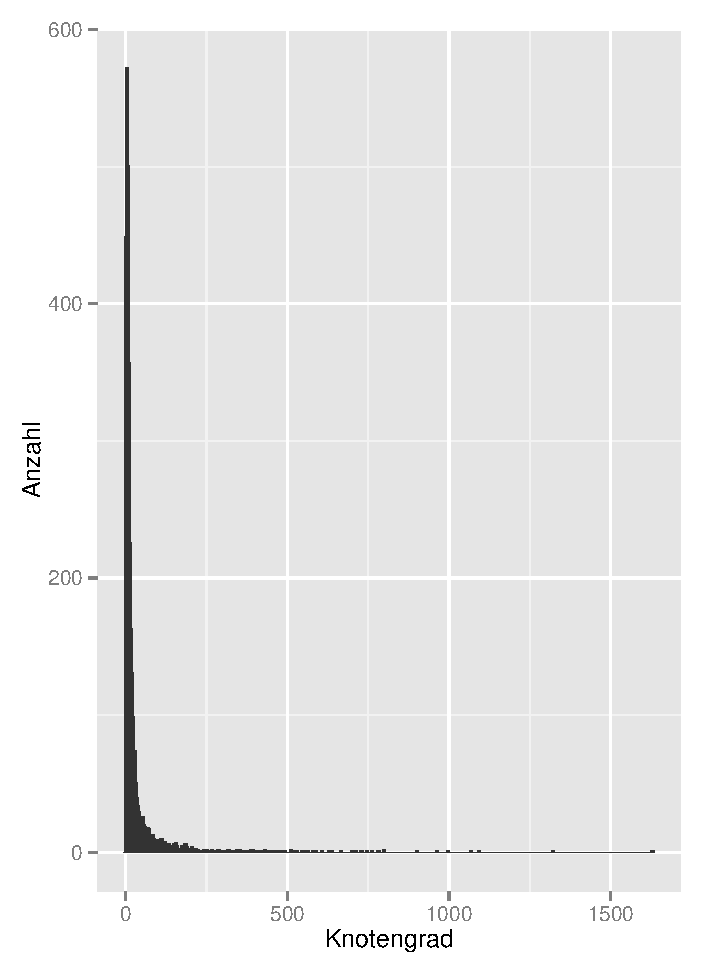
\includegraphics{testplot.pdf}

%%%%%%%%%%%%%%%%%%%%%%%%%%%%%%%%%%%%%%%%%%%%%%%%%%%%%%%%%%%%%%%%%%%%%%%%%%%%%%%%

\section{Versionshinweise}

\newpage
\begin{thebibliography}{9}
	\bibitem{Hu2005} Yifan Hu, Efficient and High Quality Force-Directed Graph, Mathematica Journal, vol. 10, Issue 1, pp. 37-71, (2005)
\end{thebibliography}
\end{document}
